\documentclass[a4paper,twoside]{report}
% notar que o relatório pode ser frente-e-verso ou apenas uma página por folha

\usepackage{relatorio} % formato ``oficial''
\usepackage[english]{babel} % para que as figuras e secções apareçam em pt
\usepackage[utf8]{inputenc} % Unicode
\usepackage{graphicx} % incluir imagens
\usepackage{url} % typeset URL's
\usepackage{textcomp} % símbolo do euro
\usepackage{multirow} % células com mais que uma linha em tabelas
\usepackage[pdftex,hidelinks]{hyperref}
\usepackage{listings}

\lstset{language=Java,breaklines=true,basicstyle=\scriptsize\ttfamily,frame=single,showstringspaces=false}
\graphicspath{ {./imagens/} }

\begin{document}
\dept{ESTIG - Escola Superior de Tecnologia e Gestão}
\course{Master in Information Systems}

\title{Meta Social Media}

\author{Carlos de Souza Lima}
\secondauthor{Leonardo Leite Meira dos Santos}
%\secauthnum{22222}

\supervisor{Prof. Paulo Matos}
% Coloca a capa, primeira página e outros

\beforepreface

\prefacesection{Abstract}
This research project aims to explore the concept of social meta-network, as a way of integrating social networks, such as Facebook, LinkedIn and others, providing an integrated perspective and transversal functionalities of added value for its users. The present approach uses graph databases, implemented using Neo4j. The nodes/vertices of the graph are used to represent people; properties on nodes are used to represent personal information of each individual; the relationships/edges represent directional relationships between individuals according to each social network; and the properties about relationships serve to maintain information about the relationship between individuals for each social network. The model created intends to be a mixed solution focused on relationships by type of social network, referring details to the information existing in the native network itself. Native networks are seen as distinct dimensions in which the present solution makes it possible to relate information between these dimensions, even when there are no relationships between the networks/user in question. It also allows for a more complete perspective of each individual, integrating the professional, playful and other more specialized aspects, which leads to results that are much higher than what can be achieved by looking individually at each network - whether for problems/challenges of centrality/influence, identification, and characterization of communities, identification of similarities, identification of potential relationships, among many other approaches. In practical terms, a considerable asset for marketing purposes.

% Coloca índices
\afterpreface

\bodystart
 
% inclusão do texto, propriamente dito
\chapter{Introduction}
\label{cha:intro}

Social media is software that is constantly present in a large part of people's lives. Nowadays contents more than 4.7 billion active users, according to \cite{statista}, which is over 93\% of the internet's users, and it tends to grow more until 2027, when this statistic will reach on 5.85 billion active users \cite{statista_util_2027}. So, it presents itself as a market in full growth that contains large companies, such as Meta owner of Facebook, Whatsapp and Instagram and also Microsoft, owner of LinkedIn. More recent emerged TikTok too, company that grown more in 2021 when grown 142\% in market value \cite{growth_tiktok}.

Therefore, the level of influence and social strength that social media has conquered to this day is perceptible. A common question is how these big companies make their money, as most of them are free. The answer to that question is not so easy and a detailed description of this subject is beyond the scope of this work. By \cite{investopedia} the highest percentage of revenue from these companies comes from Adsense. For this a fundamental resource is the large number of users and also a large dataset of their frequently use, with the objective of the Adenses to indicate a large number of people.

Otherwise, the user’s data that are maintained are also important to another functions, for example to make a recommendation of new connections or and content exhibitions. As a result of this, sometimes the data can be skewed when we consider the actives users objectives at which social media, as an example, in the most part of LinkedIn users the media are used in a professional way, meanwhile the TikTok users have an entertainment objective.

Thus, the project purpose is the construction of a system that adds information about different social medias, considering the objectives interests of every person in each networks, to do the most correct and relevant continent recommendations of connections and exhibition. This work will be followed by a mor detailed presentation of the project, and subsequently by your supplementation and presentation of the user interface idealization. Finally, having the results, they are going to be presented and after having the conclusion.


\section{Goals}

The goal of the present work is to propose a model of database to trace the profile of the users in a multisocial aspect, that is, we are researching and crossing information from different social media, taking from this a more complete profile, which can provide more accurate information. This information would be used to propose connection recommendations between different social media, based on the current connection and the interest of each person and each mapped profile.

Another goal of this work is to use the stored dataset to identify the level of influence of a person on a social media, creating a general and tag influence score, serving as parameters for choosing influential people for marketing ads on different networks.


\section{Art State}

At some related papers we may see different approaches to do the recommendations of connections in social medias. Accordingly, in \cite{multi-feature-recommendation} were is purpose a new approach to recommendations were are consider some information about the users, for example the localization, and such information are used as entries to one SVM (Support Vector Machine).

We also see an similar approach in \cite{convolutional-network}, a work in which the users information are utilized in a Convolutional Neural Network and offer as an exits better recommendations based in more complex information of the users.

While in \cite{semantic-analysis-recommendation} the work developed an algorithm of recommendation based in semantic analysis of social medias into a context of learning environments, for this the authors use some semantic web tools which assists at analysis realizations and recommendations. 

To conclude in \cite{prediction-social-network} is purposed a recommendation algorithm based on graphs, where is also done the comparison between the purposed algorithm and the traditional recommendation algorithms. 

A great difference between those works and the present one becomes from a fact that the most part of them utilize the user’s data that comes from a single social media. However much, the implementations or the utilized information vary from work to work, there wasn’t find until then one solution that are based un multiples social networks to make those recommendations. 

\chapter{Tools}

\section{Neo4J}

In order to achieve the objectives of the work, the tool chosen to provide the database is Neo4J \cite{neo4j}, which provides graph database management and is recommended for use with large volumes of data that maintain a navigational relationship between them. This database model is classified as a non-relational database, but based on graphs, that is, the database is designed on the concept of nodes and edges.

This tool allows mapping different users of different social media and their connection, in order to make extrapolations on the recommendation format. A database in the Neo4J system is composed of four main types of components, when through them it is possible to map and extract information from our databases, these components are:
\begin{itemize}
  \item Nodes: Equivalent to the vertex of the graph, being the main data within the database. They can contain information such as labels and properties.
  \item Relationship: Relationships are equivalent to the edges of a graph and describe the relationship between nodes. They can also contain properties.
  \item Labels: Labels are classifications or types of nodes, being used to categorize and classify the node into a certain type.
  \item Properties: Attributes of nodes or relationships, they are composed of key and value.
\end{itemize}
 
For graph database manipulation, Cypher \cite{cypher} is used, which is a graph manipulation language in Neo4J. Through this language we can manipulate our database in Neo4J, where we can search, insert, update and perform other functions.

\section{Python}
Python \cite{python} is a general purpose programming language that in the scope of work was used to automate processes and manipulate Neo4J, abstracting the necessary steps and also applying the necessary validations and transformations before performing the insertions.This language is also used to provide the information stored in the database through an API (Application Programming Interface), 
which makes it possible to create a graphical interface for user interactions.

\section{React}
React is a library for the JavaScript language, used to build graphical interfaces for web platforms. In the scope of this work we will use it to create the graphical interface, which accesses the API to display the information in the web system. The web interface prototype can be accessed through this \href{https://www.figma.com/file/NHTBlNSzzWVDL6fHFgLb0Q/Meta-Social-Media?node-id=0%3A1}{link}.
\chapter{Development}
The first necessarily step to the development of the work is make the abstractions, for that we classify and separate the entities, relationships and attributes of work. The data base is composed by a couple of entities called by “Social Media” and "Person", a couple types of relationship, the "HAS" to connect one person to a social network, and another relationship to represent connections type between the social networks, as the possible following labels: "PERSONAL", "INFLUENCE", "PROFESSIONAL\_RELATIONSHIP", e "CONTENTS".

Such abstractions that were citated anteriorly are codified in a program that automatize the insertion process and population of Neo4J, applying some validations and a defined logic to several connections as the verification of a relationship type, and can be find at the following \href{https://github.com/LeonardoLeiteMeira/process_CSV_to_graph_database}{repositório}. To use is necessary substitute connections data of Neo4J to the local machine.



\section{Social Medias}

The Social Media is responsible for represent one social network of one single person. A social network can be connected to many other social media and in just one person. By this way, the social networks that were chosen to be part of the project initially are currently the main utilized, being them the Instagram, Facebook, Ticktok, Youtube, Pinterest e Twitter.
The attributes of each social network are

\begin{itemize}

\item Identifier: Single identifier of the entity

\item Name: Social network name that the entity refers to 

\item User name: Responsible for identify the user name chosen by 
the person that created that social network

\item Identifier of the user: Responsible for being a reference to a person identifier ("Person" entity")

\end{itemize}




\section{Person}

The “Person” entity represent the person that utilize determinated social networks. One person can be related to many others different social networks, and yours relations with another people happen through those social networks. 

One instance of the “Person” entity have the following attributes:

\begin{itemize}
\item Identifier: A single identifier to that user
\item Name: User’s first name
\item Surname: User’s last name
\end{itemize}


\section{Relationships}


The relationships between the entities describe the behavior that are being charted by the graphs, in this case exist a couple type of present relationship at the system, one to represent the connection between one person and you social networks and another one to represent the connections between the social networks.

The first relation, between one person and tour social networks are described for the vertice “Has”, each person must be in a social network set. Were the connection are defined based at this relation. The image 3.1 shows the relation of the “Alice” person with your social networks through the vertice "HAS".  

\begin{figure}
    \centering
    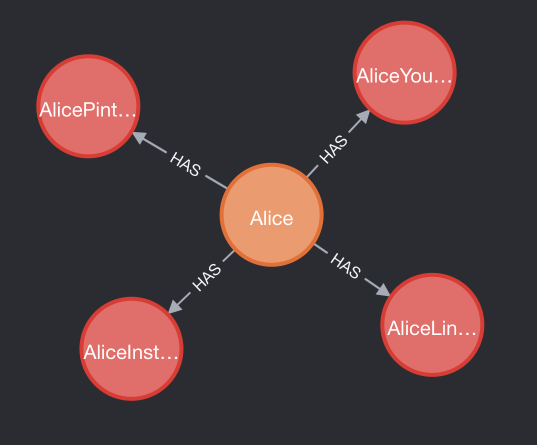
\includegraphics[scale=0.5]{alice}
    \caption{"Alice" entity with the vertices for your social networks}
    \label{fig:my_label}
\end{figure}



The other type of relationship would be one that describes the connection between two social networks of different people. This relationship takes into account the type of connection and the social networks used by two users, and can be of the following types:

\begin{itemize}
    \item Personal: Follow each other on networks for personal use
    \item Professional: Follow each other in professional networks
    \item Content consumption - Follow each other on networks focused on video content
    \item Influence: Represents the relationship of influence, when a person does not follow another but is followed by him. The vertical arrow points to who is followed, that is, who influences the relationship.
\end{itemize}



In figure 3.2 it is possible to visualize the entity "Alice" linked to the social network "AliceInstagram", and its relationship with other social networks of other people.

\begin{figure}
    \centering
    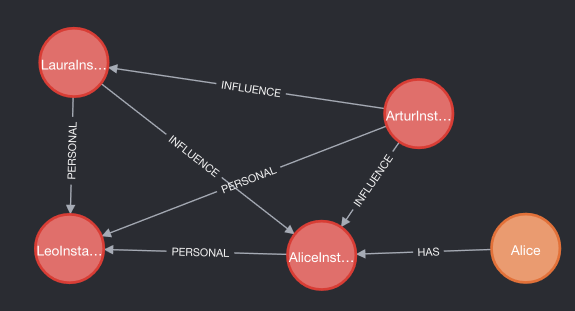
\includegraphics[scale=0.5]{imagens/alice_others.png}
    \caption{
Entity “Alice” with its social network connecting to other networks}
    \label{fig:my_label}
\end{figure}

\section{Queries}

Given the database structure presented and the objectives of this work, some queries were created in Cypher to return the desired information. The querie below returns the social media of a given person. In the example, you are looking for a person's social networks with the "Name" property as "Laura".
\begin{verbatim}
match(person:Person {Name: "Laura"})-[HAS]->(socialMedia:SocialMedia) 
return socialMedia
\end{verbatim}


The next query is intended to return all people connected to someone else's social networks. In the example, the query is looking for people connected to a person's social networks with the "Name" property as "Laura".

\begin{verbatim}
match(p:Person{Name:"Laura"})-[]-(s:SocialMedia)
match(s)-[]-(sl:SocialMedia)
match(sl)<-[HAS]-(f:Person)
return f
\end{verbatim}

The following query looks for the first-level connections for a relationship type. In the example, it searches for people who have a social network (in this case, instagram), then it searches for the social networks connected in a type of relationship (in the example, the relationship is "PERSONAL"), and finally, it searches for the social networks connected to a person (in the Leonardo case). With this query it is possible to list all connections for a type of relationship that has been identified.

\begin{verbatim}
match (p:Person)-[]-(s:SocialMedia{Name:"Instagram"})
match (s)-[f:PERSONAL]-(sl)
match (sl)-[:HAS]-(se:Person{Name:"Leonardo"})
return p
\end{verbatim}

The following query performs an in-depth search using the plugion APOC \cite{apoc} available in the Neo4J system. In the first line, the social network with “Name” defined as “Instagram” of the person “Alice“ is selected. In the second line, the search for node S (Alice's Instagram) begins, then the search for vertices is performed, with a maximum depth of 5. The result of this query are the suggestions of possible new connections of a personal nature that can be made .

\begin{verbatim}
match (p:Person{Name:"Alice"})-[]-(s:SocialMedia{Name:"Instagram"})
call apoc.path.spanningTree(s,{relationshipFilter: "PERSONAL",minLevel:0,maxLevel: 5})
YIELD path
RETURN path, p;
\end{verbatim}

For other types of recommendations just replace the "relationshipFilter" property to "INFLUENCE", to have influence recommendations, to "PROFESSIONAL\_RELATIONSHIP" to have professional connection recommendations, or "CONTENTS" to have content recommendations.


The following query is intended to return the influence score that a given person has. In the example below, all of a person's social networks are selected, in this case "Alice", and then the number of influence connections is returned.

\begin{verbatim}
match(person:Person {Name: "Alice"})-[HAS]->(socialMedia:SocialMedia)
match(socialMedia)<-[f:INFLUENCE]-()
return count(f)
\end{verbatim}


This last query aims to identify someone's level of influence within a network. In the first line, the social networks of a person are selected to be evaluated for influence. In the second line, all the social networks of a network that must be evaluated, which are influenced are selected, and finally it is defined which network the level of influence is being evaluated, in this case a social network with the property "Username" with the value " LauraInstagram”.
\begin{verbatim}
match(person:Person {Name: "Leonardo"})-[HAS]->(socialMedia:SocialMedia)
match(socialMedia)<-[f:INFLUENCE]-(socialMediaInOtherSubGraph:SocialMedia)
match(socialMediaInOtherSubGraph:SocialMedia)-
    []-(subGraph:SocialMedia{Username:"LauraInstagram"})

return count(f)
\end{verbatim}







% listagem de referências
\bibliography{refs}
% estilo de referências. outros valores posíveis são 'plain' e 'abbrv'
\bibliographystyle{ieeetr}

% Apêndice 
%\appendix
%\include{apendice}

\end{document}
